\projecthead{05 / Robotics}{Batman}{Autonomous trash-pickup robot}{SBU Hacks 2026}
\textit{Team prototype}
\par\medskip A low-cost robot designed to find and collect campus litter, bringing computer vision, omnidirectional motion, and a two-servo claw into one hardware prototype.
\par\smallskip {\small\color{muted} Tools: Arduino UNO Q, Ultralytics YOLO11, Python, mecanum drive, TCP / Wi-Fi}
\medskip
\noindent
\begin{minipage}[t]{.48\linewidth}\centering\vspace{0pt}
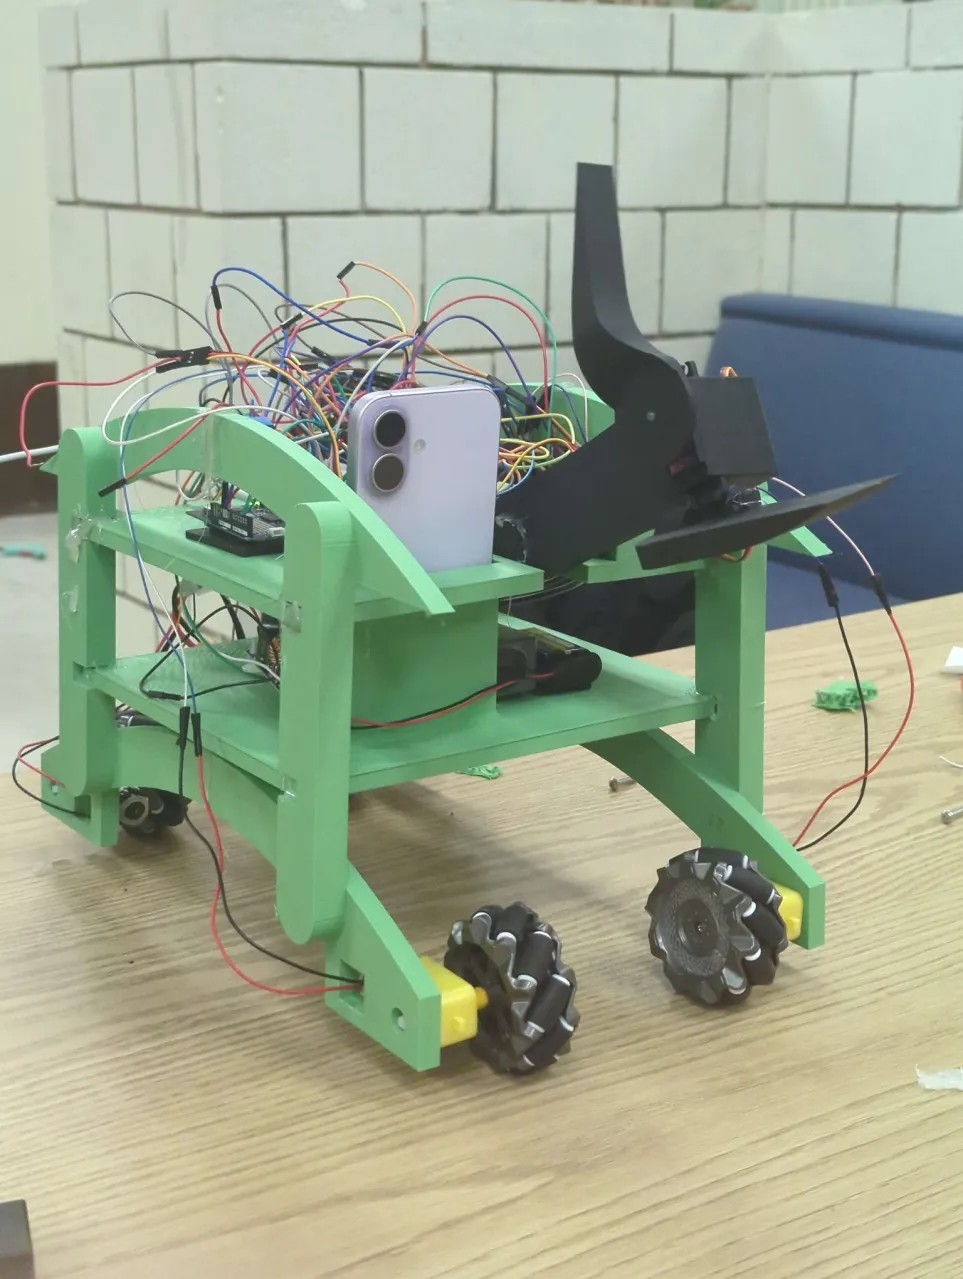
\includegraphics[width=\linewidth,height=1.8in,keepaspectratio]{images/batman/prototype.jpg}
\par\smallskip{\footnotesize\color{muted} The assembled prototype: mecanum base, iPhone camera, and two-servo claw.}\end{minipage}\hfill
\begin{minipage}[t]{.48\linewidth}\centering\vspace{0pt}
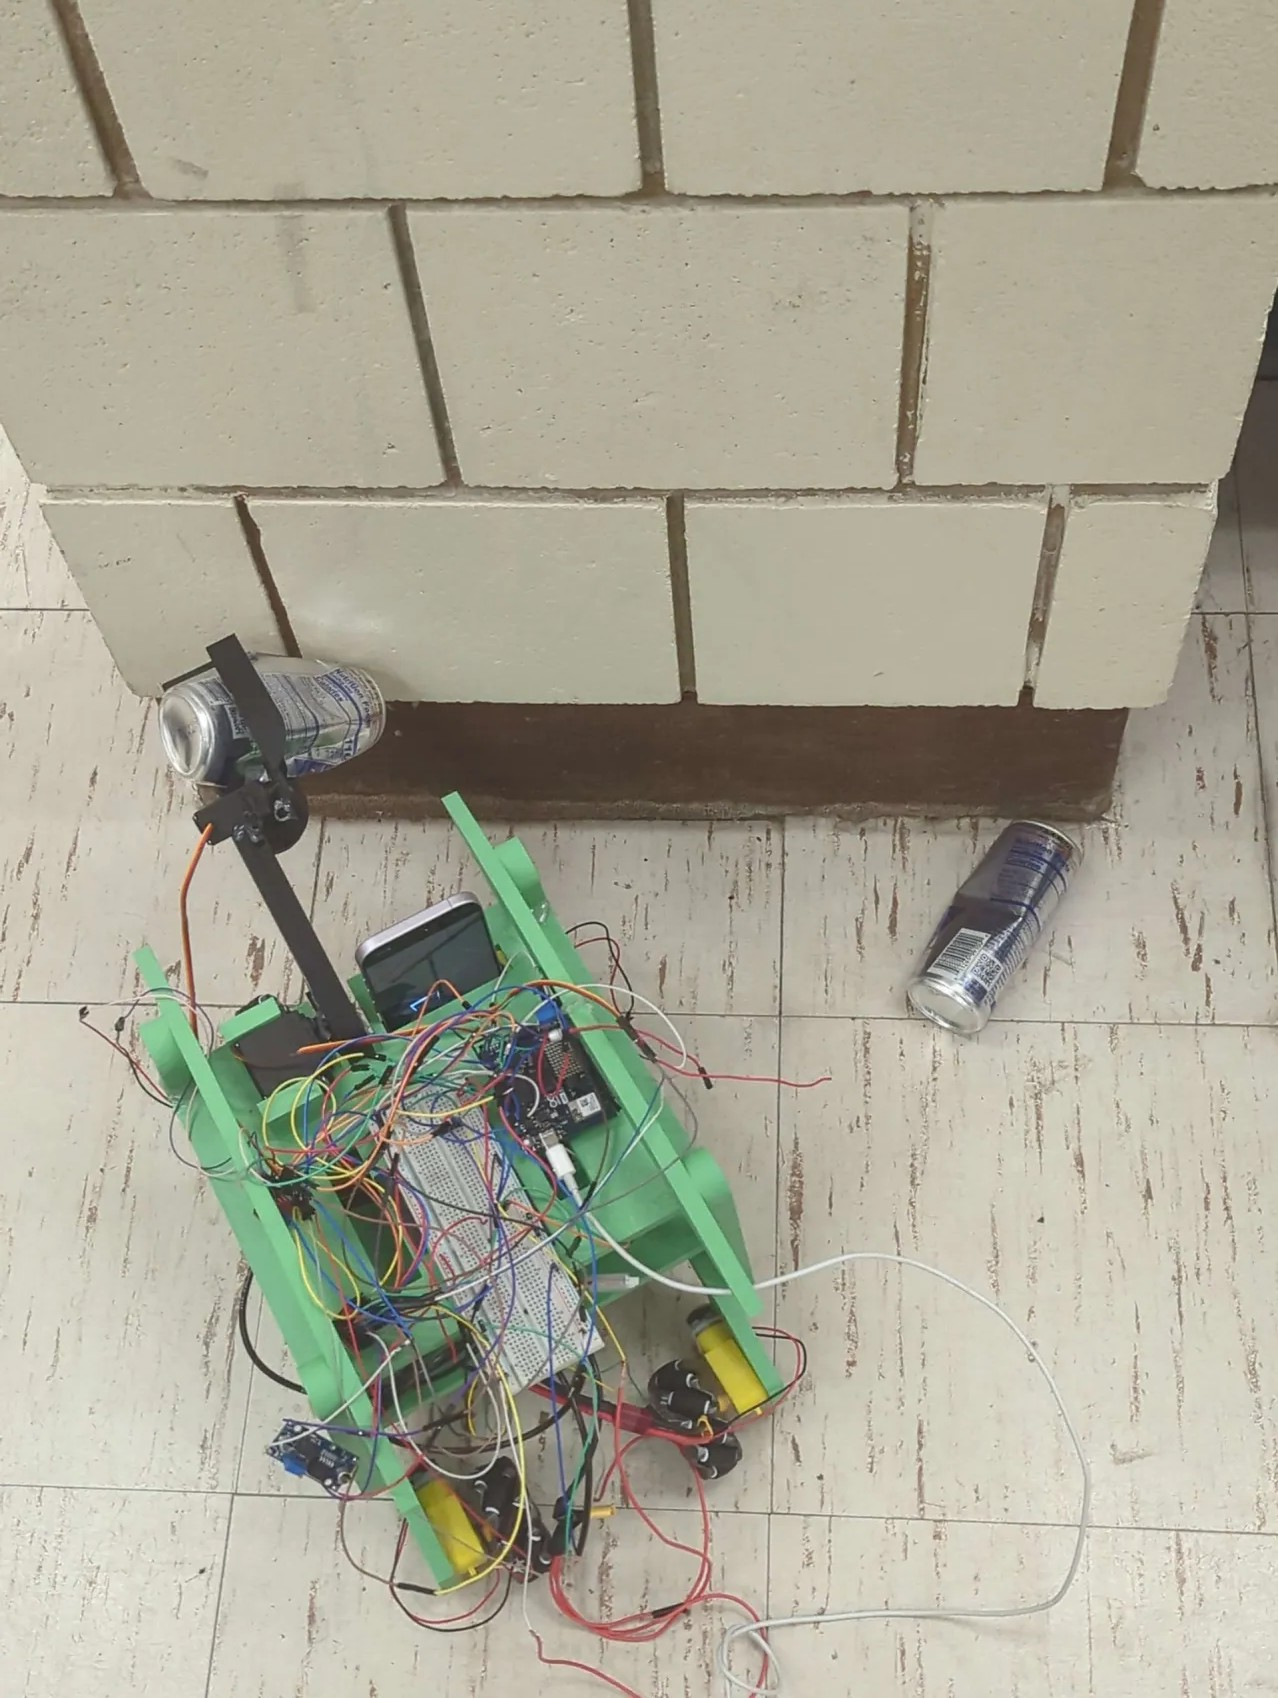
\includegraphics[width=\linewidth,height=1.8in,keepaspectratio]{images/batman/pickup-test.jpg}
\par\smallskip{\footnotesize\color{muted} Claw and chassis during a can-pickup test.}\end{minipage}\hfill
\par\medskip
\noindent
\begin{minipage}[t]{.48\linewidth}\centering\vspace{0pt}
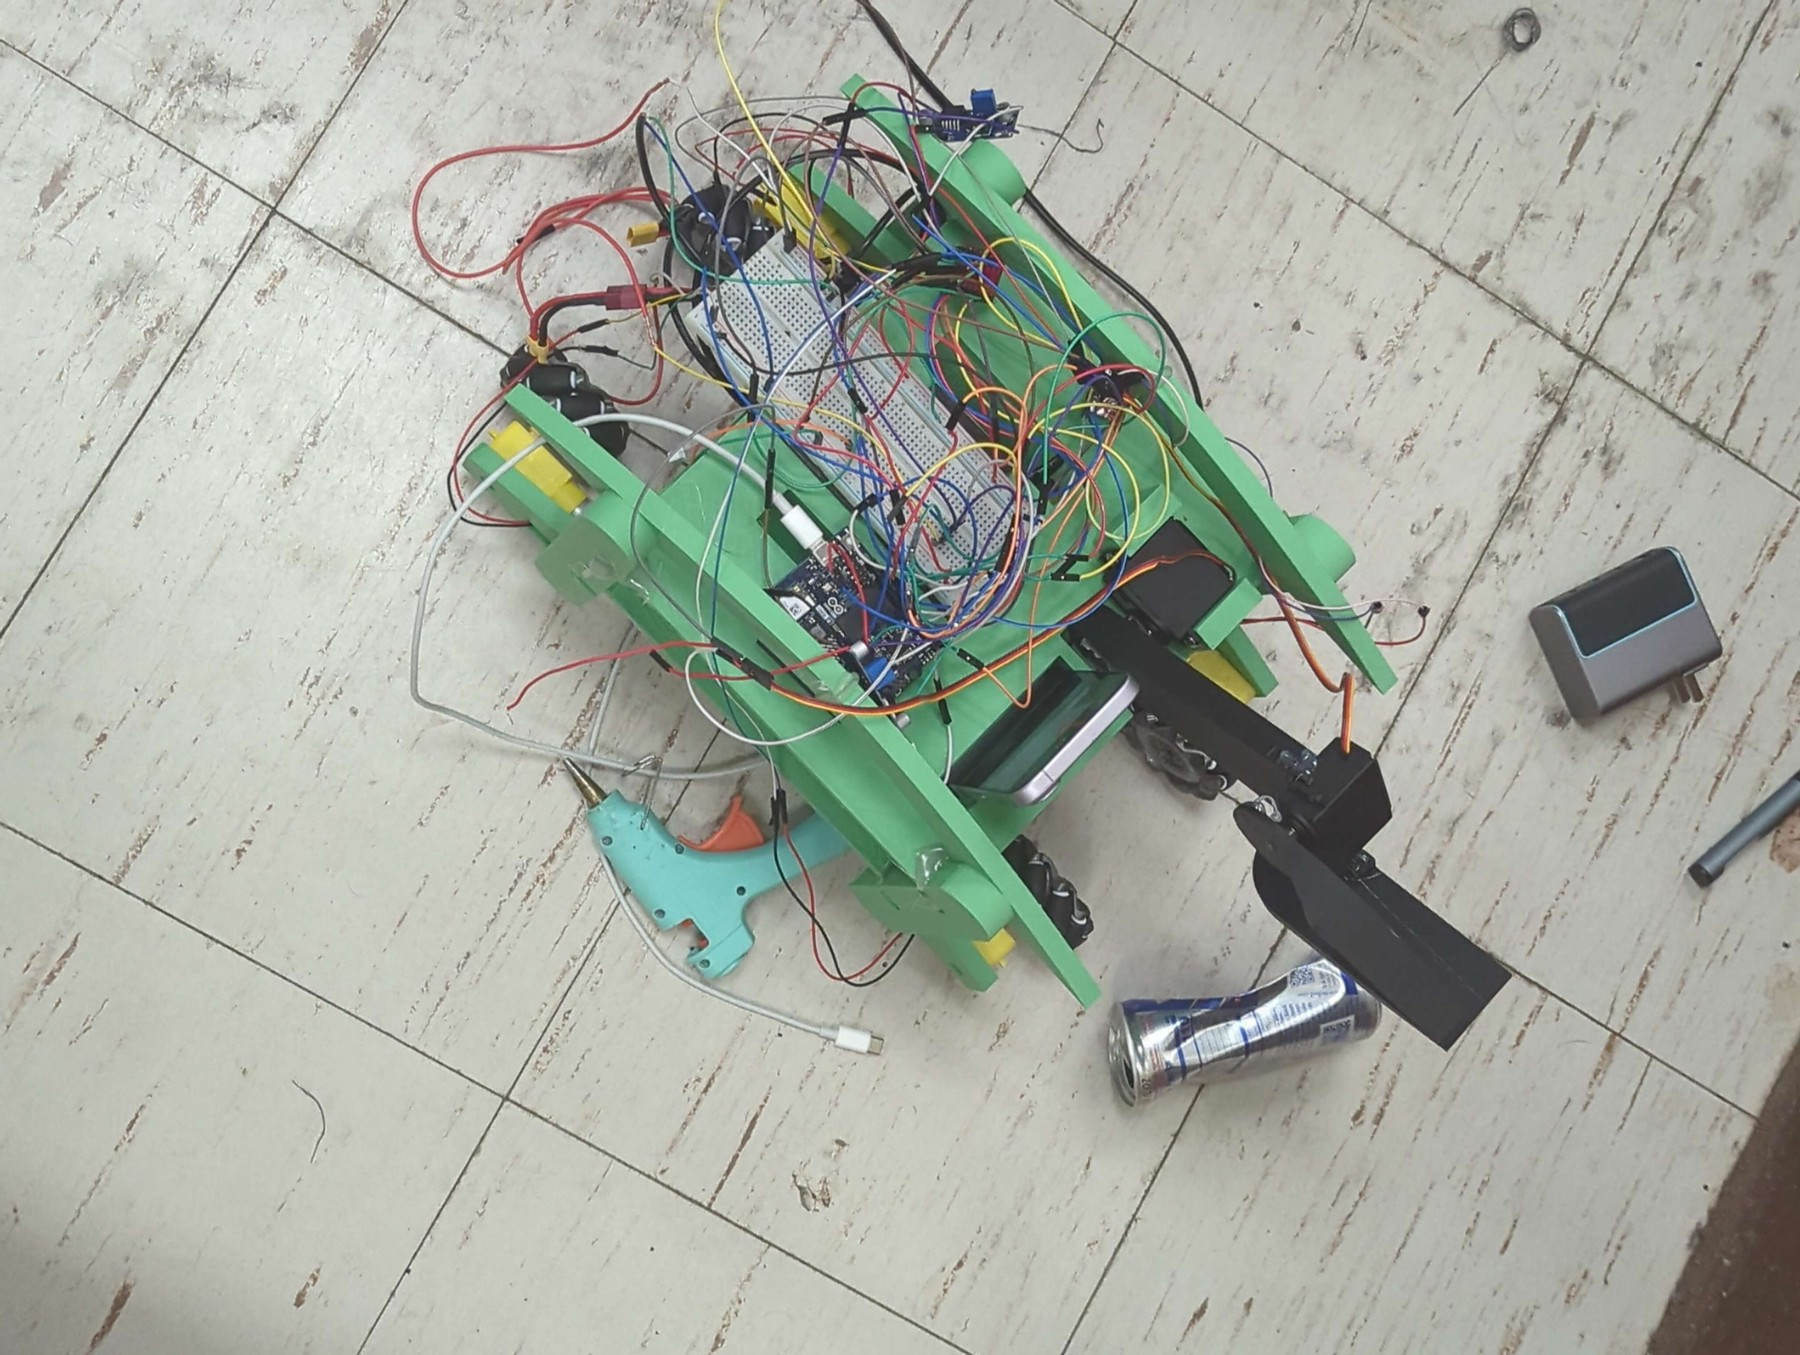
\includegraphics[width=\linewidth,height=1.8in,keepaspectratio]{images/batman/electronics.jpg}
\par\smallskip{\footnotesize\color{muted} UNO Q, breadboards, motor wiring, and arm integration.}\end{minipage}\hfill
\begin{minipage}[t]{.48\linewidth}\centering\vspace{0pt}
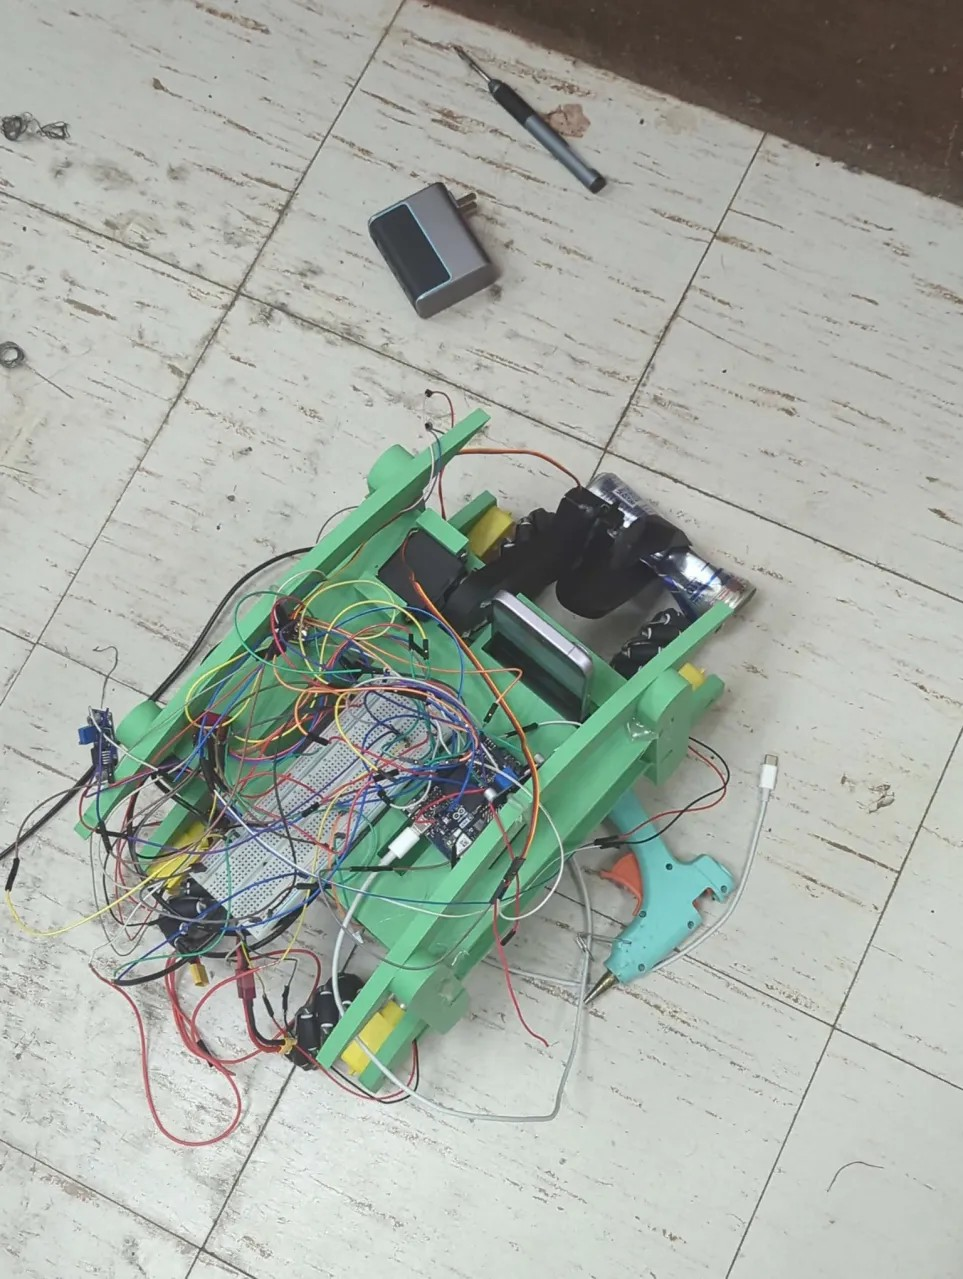
\includegraphics[width=\linewidth,height=1.8in,keepaspectratio]{images/batman/assembly.jpg}
\par\smallskip{\footnotesize\color{muted} Hardware assembly and wiring.}\end{minipage}\hfill
\par\medskip
\noindent
\begin{minipage}[t]{.48\linewidth}\centering\vspace{0pt}
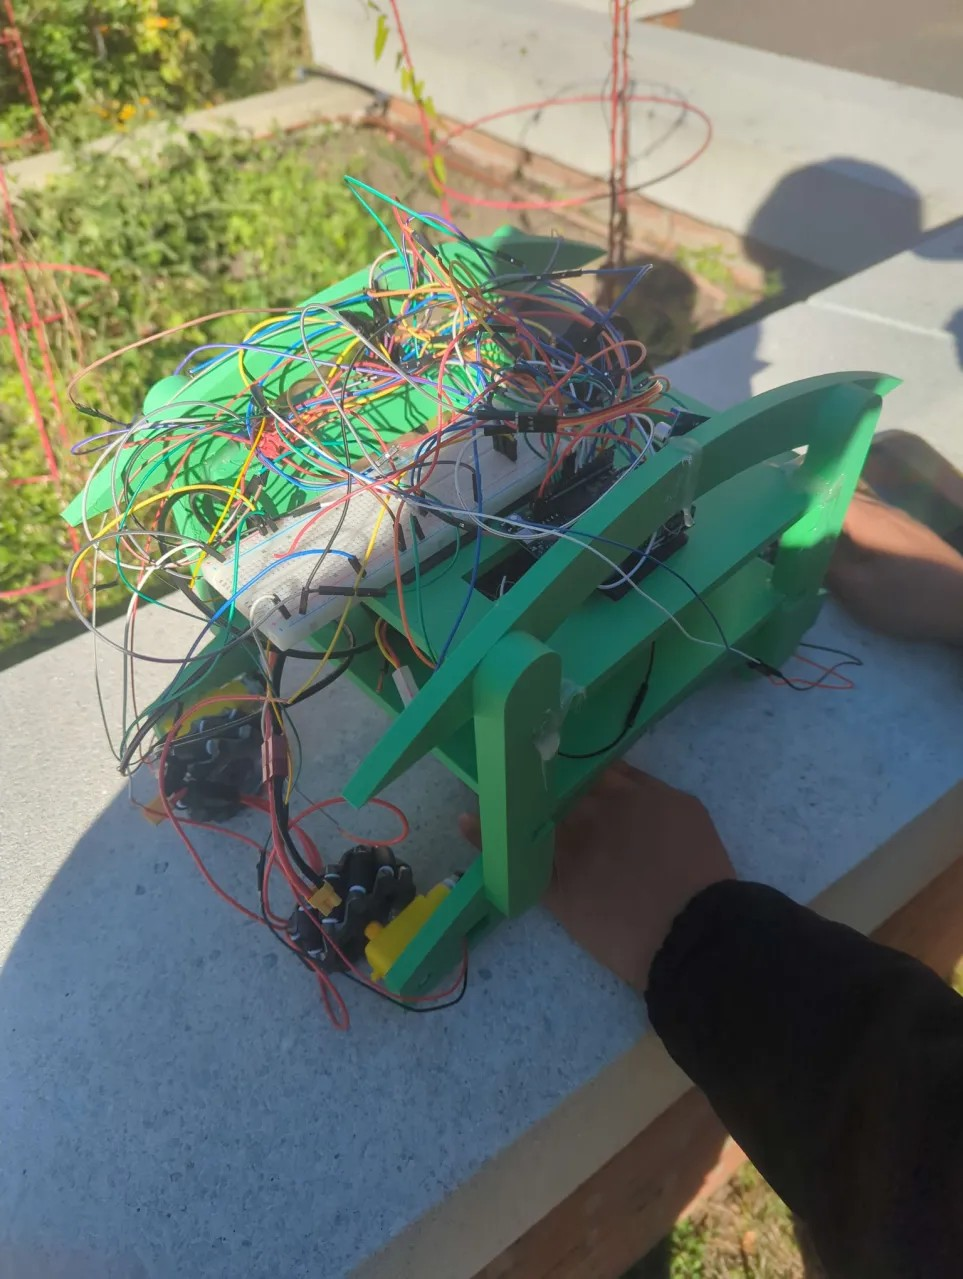
\includegraphics[width=\linewidth,height=1.8in,keepaspectratio]{images/batman/outdoor-build.jpg}
\par\smallskip{\footnotesize\color{muted} The green chassis and electronics outdoors.}\end{minipage}\hfill
\par\medskip
\subsection*{The idea}
Litter collects under benches, beside bins, and along campus walkways. Our team built Batman to explore a small, affordable robot that can reach those spots and pick it up.
\subsection*{See, decide, move, grab}
An iPhone streams video to a Windows laptop running a trash-trained YOLO11 model on an RTX 5060. Drive and arm commands travel over TCP on a shared hotspot to the UNO Q. Four motors and two HW-166 (TB6612) drivers power the mecanum base; lift and gripper servos operate the claw.
\subsection*{Integration \& lessons}
We tested the motors and servos separately before integrating vision. Stable logic power and a common ground resolved driver issues. The stock Zephyr core lacked Servo.h, so the team used soft 50 Hz servo pulses. A shared hotspot replaced campus Wi-Fi for the robot link.
\subsection*{Current state \& next steps}
The physical base, arm controller, and GPU detector are built. Reliable pickup remains a tuning task: center on detections, improve the grab sequence, tidy the harness, and extend battery runs. Obstacle sensing and onboard compute are future options.
\medskip\href{https://github.com/muhammadmaalik/Batman}{View repository}